
%\documentclass[mathserif]{beamer}
\documentclass[handout]{beamer}
%\usetheme{Goettingen}
%\usetheme{Warsaw}
\usetheme{Singapore}



%\usetheme{Frankfurt}
%\usetheme{Copenhagen}
%\usetheme{Szeged}
%\usetheme{Montpellier}
%\usetheme{CambridgeUS}
%\usecolortheme{}
%\setbeamercovered{transparent}
\usepackage[english, activeacute]{babel}
\usepackage[utf8]{inputenc}
\usepackage{amsmath, amssymb}
\usepackage{dsfont}
\usepackage{graphics}
\usepackage{cases}
\usepackage{graphicx}
\usepackage{pgf}
\usepackage{epsfig}
\usepackage{amssymb}
\usepackage{multirow}	
\usepackage{amstext}
\usepackage[ruled,vlined,lined]{algorithm2e}
\usepackage{amsmath}
\usepackage{epic}
\usepackage{epsfig}
\usepackage{fontenc}
\usepackage{framed,color}
\usepackage{palatino, url, multicol}
%\algsetup{indent=2em}
\newcommand{\factorial}{\ensuremath{\mbox{\sc Factorial}}}
\newcommand{\BIGOP}[1]{\mathop{\mathchoice%
{\raise-0.22em\hbox{\huge $#1$}}%
{\raise-0.05em\hbox{\Large $#1$}}{\hbox{\large $#1$}}{#1}}}
\newcommand{\bigtimes}{\BIGOP{\times}}
\vspace{-0.5cm}
\title{Natural Language Processing \\ Contextualized Embeddings, Pre-Training, Fine-Tuning and Large Language Models}
\vspace{-0.5cm}
\author[Felipe Bravo Márquez]{\footnotesize
%\author{\footnotesize  
 \textcolor[rgb]{0.00,0.00,1.00}{Felipe Bravo-Marquez}} 
  
 

\date{\today}

\begin{document}
\begin{frame}
\titlepage


\end{frame}



\begin{frame}{Representations for a word}
\begin{scriptsize}
\begin{itemize}
\item So far, we've basically had one representation of words, the word embeddings we've already learned:  Word2vec, GloVe, fastText.\footnote{These slides are based on the Stanford CS224N: Natural Language Processing with Deep Learning course: \url{http://web.stanford.edu/class/cs224n/}}.
\item These embeddings have a useful semi-supervised quality, as they can be learned from unlabeled corpora and used in our downstream task-oriented architectures (LSTM, CNN, Transformer).

\item However, they exhibit two problems.
\item  Problem 1: They always produce the same representation for a word type regardless of the context in which a word token occurs
\item  We might want very fine-grained word sense disambiguation
\item Problem 2: We just have one representation for a word, but words have different aspects, including semantics, syntactic behavior, and register/connotations

 

\end{itemize}
\end{scriptsize}
\end{frame}

\begin{frame}{Neural Language Models can produce Contextualized Embeddings}
\begin{scriptsize}
\begin{itemize}
\item In, a Neural Language Model (NLM), we immediately stuck word vectors (perhaps only trained on the corpus) through LSTM layers
\item  Those LSTM layers are trained to predict the next word.
\item  But these language models produce context-specific word representations in the hidden states of each position.

    \begin{figure}[h]
        	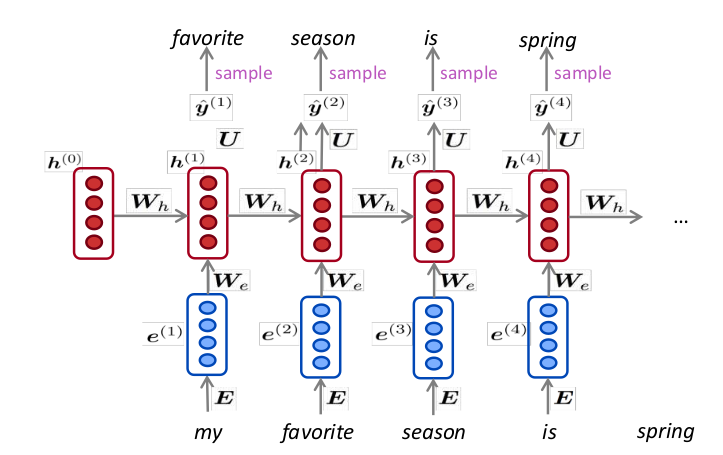
\includegraphics[scale = 0.4]{pics/lstm_nlm.png}
        \end{figure}  


\end{itemize}
\end{scriptsize}
\end{frame}




\begin{frame}{ELMo: Embeddings from Language Models}
\begin{scriptsize}
\begin{itemize}
\item Idea: train a large language model (LM)  with a recurrent neural network and use its hidden states as ``contextualized word embeddings'' 
\cite{peters-etal-2018-deep}. 

\item ELMO is bidirectional LM with 2 biLSTM layers and around 100 million parameters.
\item  Uses character CNN to build initial word representation (only)
\item  2048 char n-gram filters and 2 highway layers, 512 dim projection
\item  User 4096 dim hidden/cell LSTM states with 512 dim projections to next input
\item  Uses a residual connection
\item  Parameters of token input and output (softmax) are tied.


 

\end{itemize}
\end{scriptsize}
\end{frame}


\begin{frame}{ELMo: Embeddings from Language Models}
    \begin{figure}[h]
        	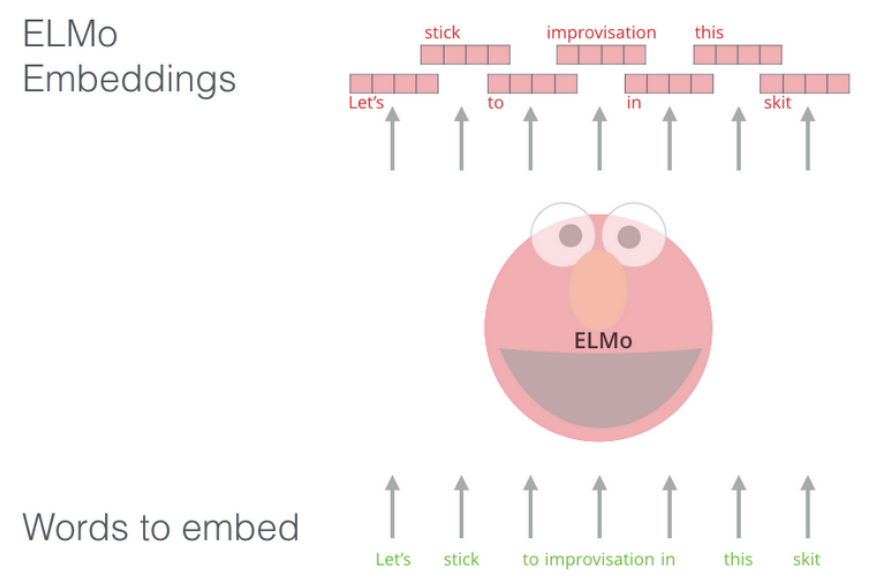
\includegraphics[scale = 0.29]{pics/elmo.png}
        \end{figure}  
\end{frame}



\begin{frame}{ELMo: Use with a task}
\begin{scriptsize}
\begin{itemize}
\item First run biLM to get representations for each word.
\item Then let (whatever) end-task model use them.
\item  Freeze weights of ELMo for purposes of supervised model.
\item  Concatenate ELMo weights into task-specific model.


    \begin{figure}[h]
        	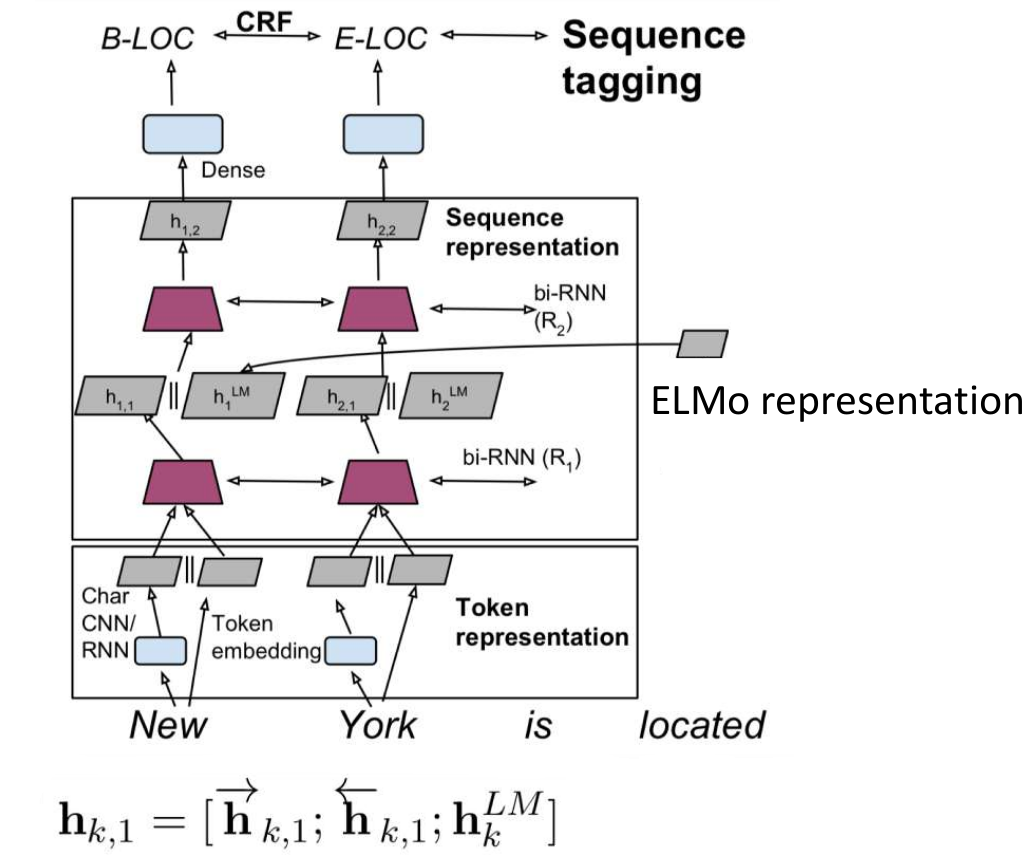
\includegraphics[scale = 0.25]{pics/elmo2.png}
        \end{figure}  

 

\end{itemize}
\end{scriptsize}
\end{frame}

\begin{frame}{ELMo: Results}

    \begin{figure}[h]
        	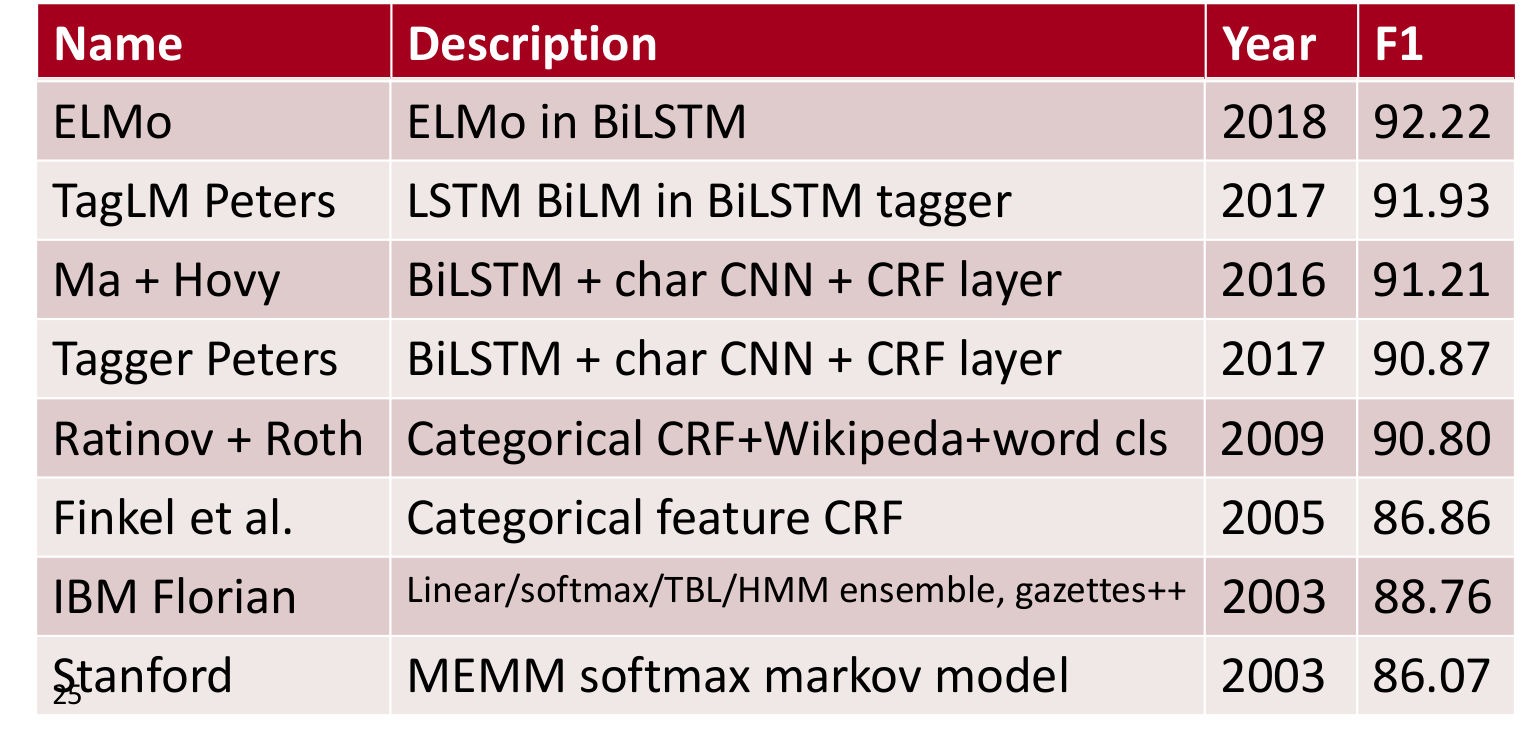
\includegraphics[scale = 0.25]{pics/elmo_results.png}
        \end{figure}  

 


\end{frame}


\begin{frame}{ULMfit}
\begin{scriptsize}
\begin{itemize}
\item Howard and Ruder (2018) Universal Language Model Fine-tuning for Text Classification \cite{howard-ruder-2018-universal}. 
\item Same general idea of transferring NLM knowledge
\item  Here applied to text classification

\begin{figure}[h]
        	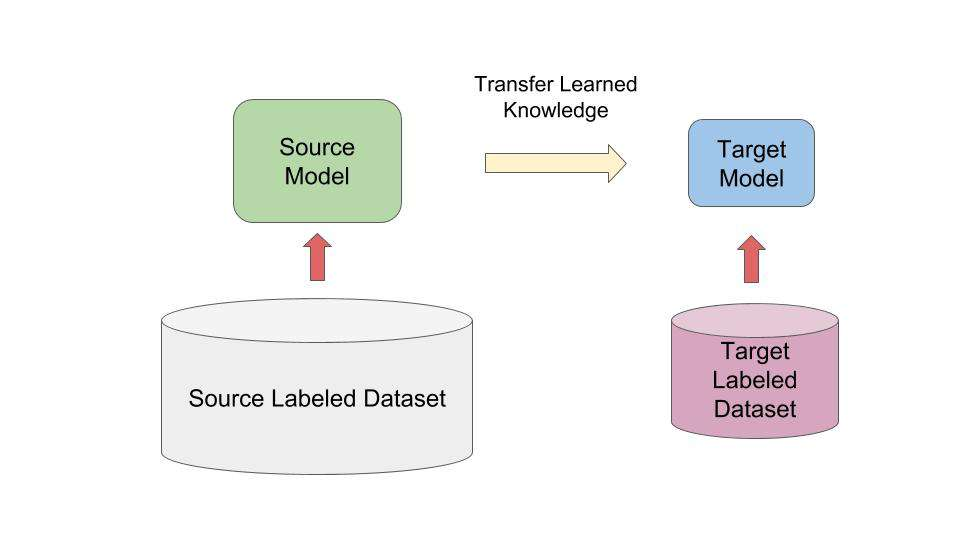
\includegraphics[scale = 0.29]{pics/ulmfit1.png}
        \end{figure}  

\end{itemize}
\end{scriptsize}
\end{frame}


\begin{frame}{ULMfit}
\begin{scriptsize}
\begin{itemize}
\item Train LM on big general domain corpus (use biLM)
\item Tune LM on target task data
\item Fine-tune as classifier on target task

\begin{figure}[h]
        	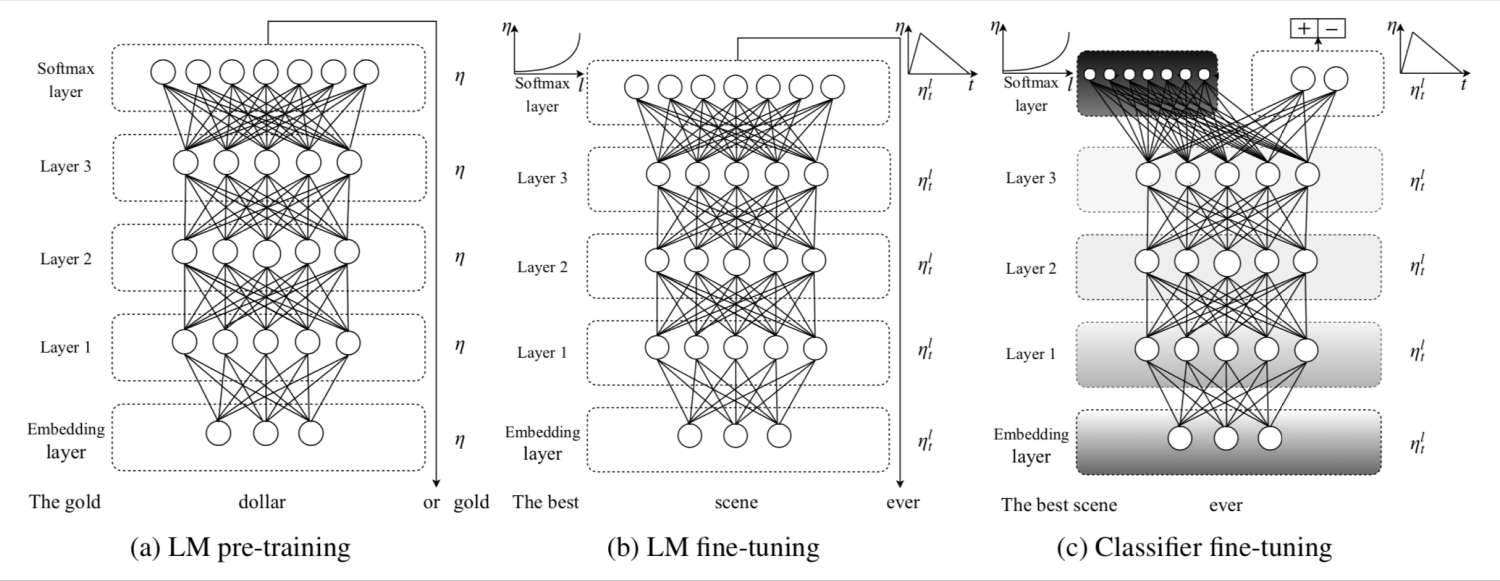
\includegraphics[scale = 0.2]{pics/ulmfit2.png}
        \end{figure}  

\end{itemize}
\end{scriptsize}
\end{frame}


\begin{frame}{ULMfit emphases}
\begin{scriptsize}
\begin{itemize}
\item Use reasonable-size ``1 GPU'' language model not really huge one
\item A lot of care in LM fine-tuning
\item Different per-layer learning rates
\item Slanted triangular learning rate (STLR) schedule
\item Gradual layer unfreezing and STLR when learning classifier
\item Classify using concatenation $[h_T, $maxpool$(h),$meanpool$(h)]$

\begin{figure}[h]
        	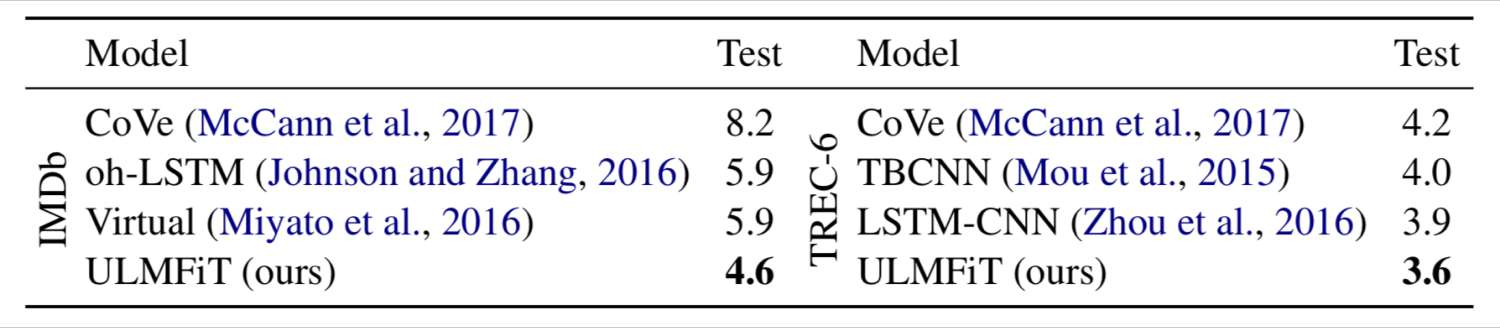
\includegraphics[scale = 0.2]{pics/ulmfit3.png}
        	Text classifier error rates
        \end{figure}  

\end{itemize}
\end{scriptsize}
\end{frame}




\begin{frame}{ULMfit transfer learning}

\begin{figure}[h]
        	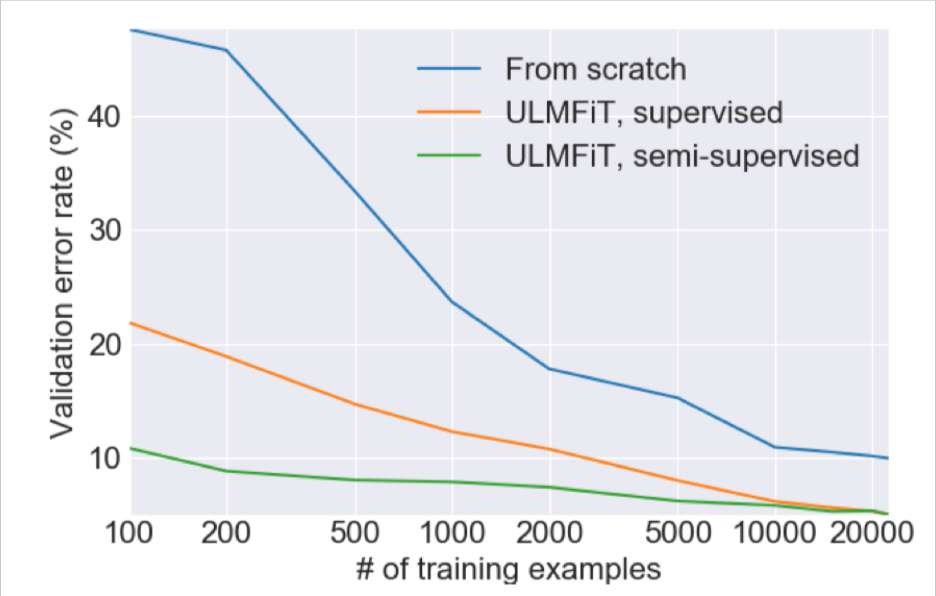
\includegraphics[scale = 0.3]{pics/ulmfit4.png}
        \end{figure}  


\end{frame}


\begin{frame}{Let’s scale it up!}


     \begin{figure}[h]
        	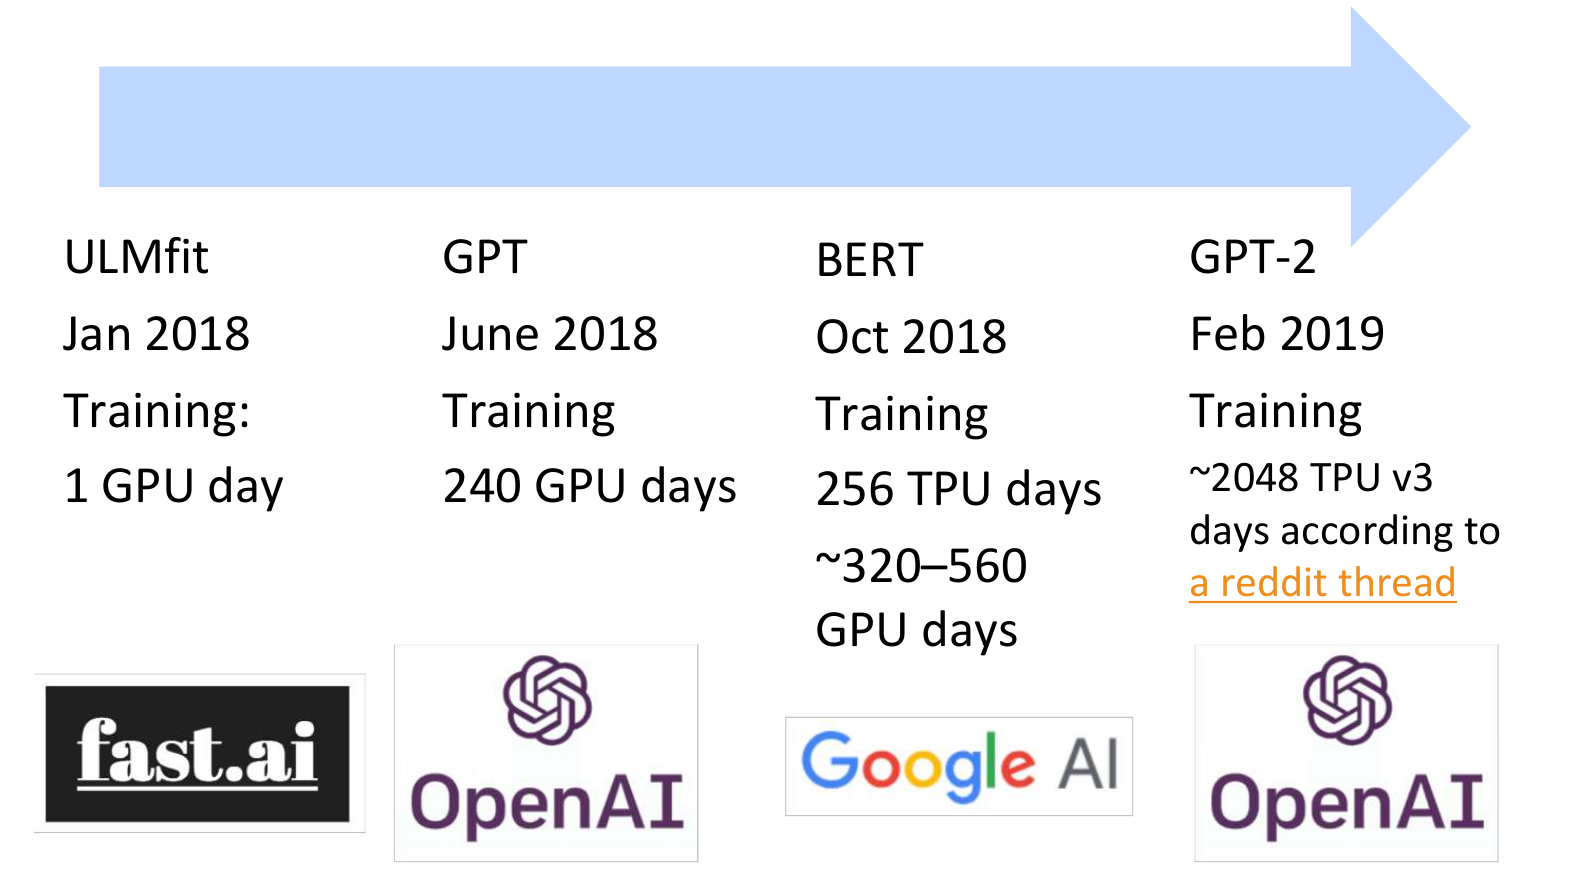
\includegraphics[scale = 0.28]{pics/llmscale.png}
        \end{figure}  


\end{frame}


\begin{frame}{GPT-2 language model (cherry-picked) output}
\begin{scriptsize}


\textbf{Human provided prompt}:

In a shocking finding, scientist discovered a herd of unicorns living in a remote, previously unexplored valley, in the Andes Mountains. Even more surprising to the researchers was the fact that the unicorns spoke perfect English. \\ 
\textbf{Model Completition}: \\ 

The scientist named the population, after their distinctive horn, Ovid’s Unicorn. These four-horned, silver-white unicorns were previously unknown to science.

Now, after almost two centuries, the mystery of what sparked this odd phenomenon is finally solved.

Dr. Jorge Pérez, an evolutionary biologist from the University of La Paz, and several companions, were exploring the Andes Mountains when they found a small valley, with no other animals or humans. Pérez noticed that the valley had what appeared to be a natural fountain, surrounded by two peaks of rock and silver snow.


\end{scriptsize}
\end{frame}

\begin{frame}{Transformer models}


     \begin{figure}[h]
        	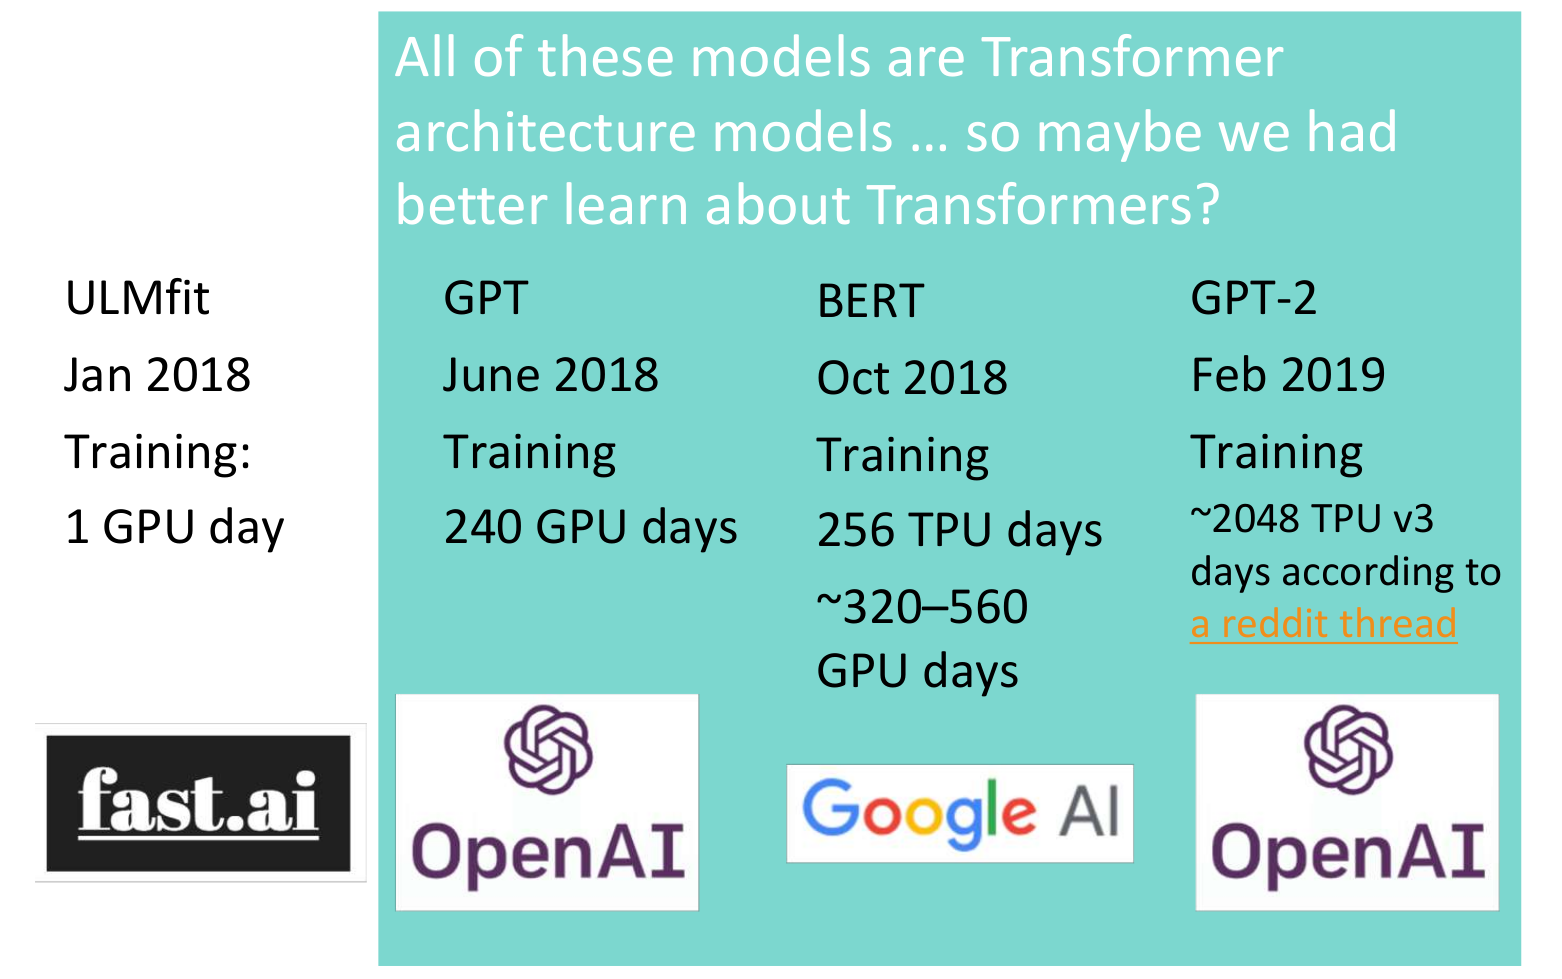
\includegraphics[scale = 0.28]{pics/llmscale_trans.png}
        \end{figure}  


\end{frame}

\begin{frame}{BERT (Bidirectional Encoder Representations from Transformers)}
\begin{scriptsize}
\begin{itemize}
\item Idea: combine ideas from ELMO, ULMFit and the Transformer \cite{kenton2019bert}.
\item How: Train a large model (335 million parameters) from a large unlabeled corpus using a Transformer encoder and then fine-tune it for other downstream tasks.
\item The parallelizable properties of the Transformer (unlike RNNs, which must be processed sequentially) allow the model to scale to more parameters.
\item This model is related but a little bit different from a standard Language Model.

     \begin{figure}[h]
        	
\includegraphics[scale = 0.4]{pics/bert.png}
        \end{figure}  




\end{itemize}
\end{scriptsize}
\end{frame}


\begin{frame}
\frametitle{Questions?}
%\vspace{1.5cm}
\begin{center}\LARGE Thanks for your Attention!\\ \end{center}



\end{frame}

\begin{frame}[allowframebreaks]\scriptsize
\frametitle{References}
\bibliography{bio}
\bibliographystyle{apalike}
%\bibliographystyle{flexbib}
\end{frame}  


%%%%%%%%%%%%%%%%%%%%%%%%%%%

\end{document}
